\documentclass[12pt,a4paper]{article}

%% ─── Packages ────────────────────────────────────────────────────────────────
\usepackage[margin=1in,headheight=15pt]{geometry}
\usepackage{amsmath, amssymb}
\usepackage{graphicx}
\usepackage{booktabs}
\usepackage{array}
\usepackage{tabularx}
\usepackage{xcolor}
\usepackage{hyperref}
\usepackage{enumitem}
\usepackage{fancyhdr}
\usepackage{titlesec}
\usepackage{caption}
\usepackage{subcaption}
\usepackage{float}
\usepackage{mdframed}
\usepackage{setspace}
\usepackage{url}
\usepackage{microtype}

%% ─── Colours ──────────────────────────────────────────────────────────────────
\definecolor{navyblue}{RGB}{31,56,100}
\definecolor{midblue}{RGB}{46,80,144}
\definecolor{lightblue}{RGB}{232,240,251}
\definecolor{warnyellow}{RGB}{255,243,205}

%% ─── Hyperlinks ───────────────────────────────────────────────────────────────
\hypersetup{
  colorlinks=true,
  linkcolor=midblue,
  citecolor=midblue,
  urlcolor=midblue,
  pdftitle={The Spatial Generalisation Problem in Vision Transformers},
  pdfauthor={Poreddy Srivatsav Reddy},
}

%% ─── Section heading styles ──────────────────────────────────────────────────
\titleformat{\section}
  {\large\bfseries\color{navyblue}}{\thesection}{1em}{}[{\color{midblue}\titlerule[0.6pt]}]
\titleformat{\subsection}
  {\normalsize\bfseries\color{midblue}}{\thesubsection}{1em}{}
\titleformat{\subsubsection}
  {\normalsize\bfseries\color{navyblue}}{\thesubsubsection}{1em}{}

\titlespacing{\section}{0pt}{14pt}{6pt}
\titlespacing{\subsection}{0pt}{10pt}{4pt}

%% ─── Callout box environments ─────────────────────────────────────────────────
\newmdenv[
  backgroundcolor=lightblue,
  linecolor=midblue,
  linewidth=1.2pt,
  leftline=true, rightline=false, topline=false, bottomline=false,
  innerleftmargin=10pt, innerrightmargin=10pt,
  innertopmargin=8pt, innerbottommargin=8pt,
  skipabove=8pt, skipbelow=8pt,
]{callout}

\newmdenv[
  backgroundcolor=warnyellow,
  linecolor=orange,
  linewidth=1.2pt,
  leftline=true, rightline=false, topline=false, bottomline=false,
  innerleftmargin=10pt, innerrightmargin=10pt,
  innertopmargin=8pt, innerbottommargin=8pt,
  skipabove=8pt, skipbelow=8pt,
]{warning}

%% ─── Page style ──────────────────────────────────────────────────────────────
\pagestyle{fancy}
\fancyhf{}
\rhead{\small\color{gray}Vision Transformer Positional Encoding}
\lhead{\small\color{gray}Research Problem Document}
\cfoot{\small\thepage}
\renewcommand{\headrulewidth}{0.3pt}

%% ─── Spacing ─────────────────────────────────────────────────────────────────
\setlength{\parskip}{6pt}
\setlength{\parindent}{0pt}
\onehalfspacing

%% ═══════════════════════════════════════════════════════════════════════════════
\begin{document}

%% ─── Title page ──────────────────────────────────────────────────────────────
\begin{titlepage}
  \centering
  \vspace*{1cm}
  {\small\scshape\color{gray} Research Problem Document\par}
  \vspace{0.6cm}
  {\LARGE\bfseries\color{navyblue}
    The Spatial Generalisation Problem\\[6pt]
    in Vision Transformers\par}
  \vspace{0.5cm}
  {\large\itshape\color{midblue}
    How Direct Patch-Position Assignment\\
    Prevents True Spatial Understanding\par}
  \vspace{0.8cm}
  \textcolor{gray}{\rule{0.6\linewidth}{0.4pt}}
  \vspace{0.6cm}

  {\normalsize
    \textbf{Author:} Poreddy Srivatsav Reddy\\[4pt]
    \href{mailto:poreddy.reddy@research.iiit.ac.in}%
         {poreddy.reddy@research.iiit.ac.in}\\[8pt]
    \textbf{Supervisor:} Prof.\ Praveen Paruchuri\\[4pt]
    \href{mailto:praveen.p@iiit.ac.in}{praveen.p@iiit.ac.in}\\[8pt]
    International Institute of Information Technology, Hyderabad (IIIT-H)\\[12pt]
    \today
  }

  \vspace{1cm}
  \textcolor{gray}{\rule{0.6\linewidth}{0.4pt}}
  \vspace{0.8cm}

  \begin{minipage}{0.82\linewidth}
    \small\itshape\centering
    ``Looked through the text and based on the references and info, the problem
    seems quite valid --- can be a potential problem to explore.''\\[4pt]
    \normalfont\small --- Prof.\ Praveen Paruchuri, IIIT-H (April 2026)
  \end{minipage}
\end{titlepage}

%% ─── Table of contents ───────────────────────────────────────────────────────
\tableofcontents
\newpage

%% ═══════════════════════════════════════════════════════════════════════════════
\section{Motivating Observations: A Bird Identification Case Study}
\label{sec:motivation}

The screenshots below illustrate a practical scenario in which spatial context
matters enormously for fine-grained visual recognition. Three birds ---
the \textbf{Crested Caracara}, the \textbf{King Vulture}, and the
\textbf{Andean Condor} --- are visually similar at coarse scales yet
taxonomically distinct. A model that memorises fixed patch-position statistics
will confuse them whenever the bird appears in an unexpected region or at an
unusual scale.

\begin{figure}[H]
  \centering
  \begin{subfigure}[t]{0.48\linewidth}
    
\includegraphics[width=\linewidth]{fig1.png}
    \caption{Crested Caracara --- puzzle vs.\ reference.}
    \label{fig:caracara}
  \end{subfigure}\hfill
  \begin{subfigure}[t]{0.48\linewidth}
    
\includegraphics[width=\linewidth]{fig2.png}
    \caption{King Vulture --- puzzle vs.\ reference.}
    \label{fig:kingvulture}
  \end{subfigure}

  \vspace{0.6em}

  \begin{subfigure}[t]{0.48\linewidth}
    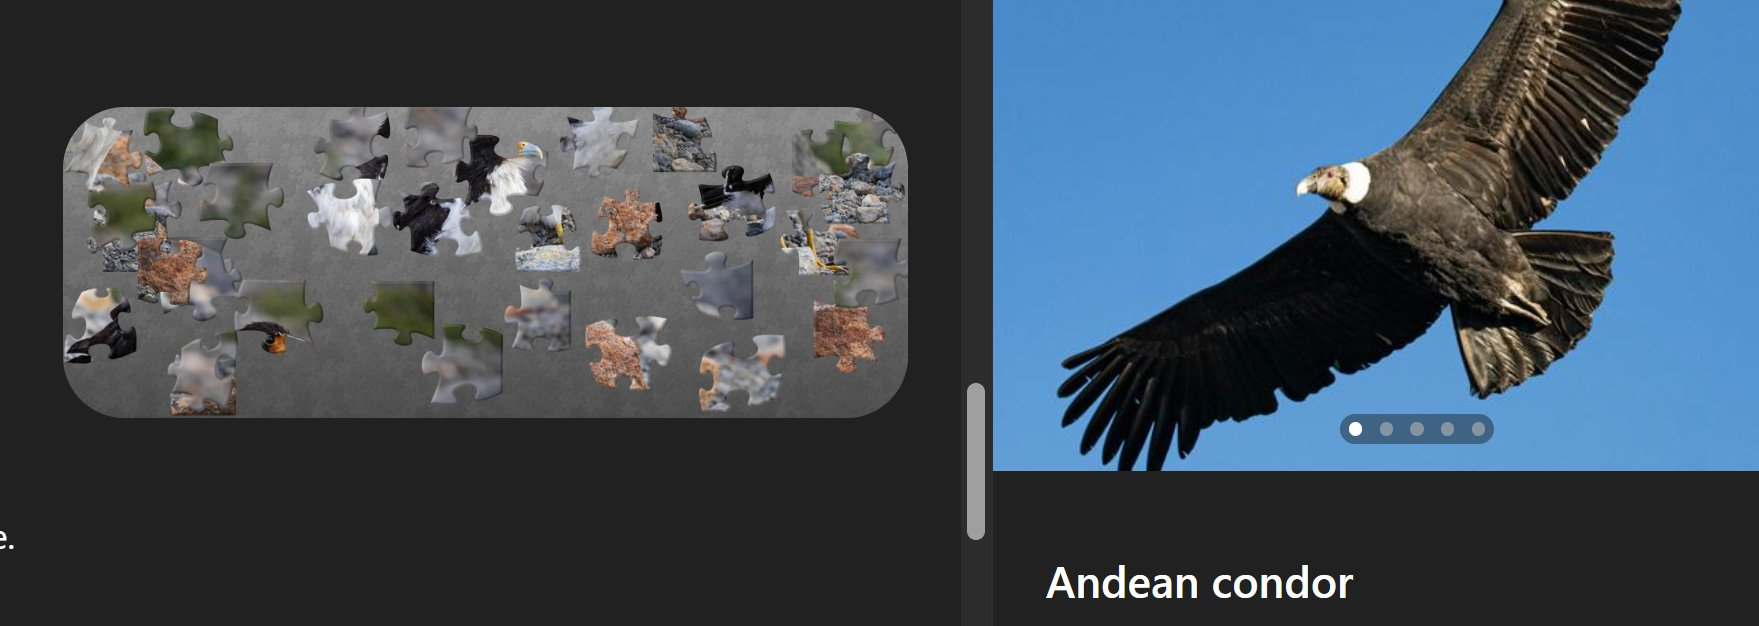
\includegraphics[width=\linewidth]{fig3.png}
    \caption{Andean Condor --- scattered puzzle pieces vs.\ reference.}
    \label{fig:condor}
  \end{subfigure}
  \caption{Bird identification under spatial disruption. Left column: puzzle
    representation (spatially disrupted patches). Right column: reference
    photograph with ground-truth label. A ViT using learned absolute positional
    embeddings struggles when patches appear in non-training positions.}
  \label{fig:birds}
\end{figure}

The figures directly motivate the core thesis: \emph{a model that binds
recognition to fixed patch positions cannot generalise when those positions
shift}.

\newpage

%% ═══════════════════════════════════════════════════════════════════════════════
\section{Abstract}

Vision Transformers (ViTs) have demonstrated impressive performance across
visual recognition tasks, yet a persistent and fundamental limitation hampers
their generalisation capability: the way spatial position is communicated to
the model. The dominant approach --- assigning each image patch a fixed,
learned positional embedding --- causes the model to \emph{memorise} spatial
locations rather than \emph{learn} structural relationships. This leads to
well-documented failures when the model encounters images at different
resolutions, different aspect ratios, or with objects shifted from their
training distribution.

This document formally defines the problem, traces its origins, surveys the
landscape of proposed solutions, assesses honestly what remains unsolved, and
positions a novel LLaMA-inspired architectural direction as a promising but
under-explored research avenue.

%% ═══════════════════════════════════════════════════════════════════════════════
\section{The Core Problem: What Exactly Is Breaking?}
\label{sec:problem}

\subsection{How ViT Assigns Position}

When an image is fed into a Vision Transformer, it is divided into a grid of
fixed-size patches. Each patch is linearly projected into an embedding
vector. To inject location awareness, Dosovitskiy et al.\ \cite{vit2020} add
a \emph{learned} positional embedding to each patch embedding:

\begin{equation}
  \mathbf{x}_i = \mathrm{patch}_i + \mathbf{p}_i
  \label{eq:absolute}
\end{equation}

where $\mathbf{p}_i$ is a trainable vector, one per patch position.
The critical detail: $\mathbf{p}_i$ is an \textbf{absolute address}.
Patch at grid position $(\mathrm{row}=3,\,\mathrm{col}=5)$ always receives
the same embedding $\mathbf{p}_{(3,5)}$, regardless of context, scale, or
content. The model has no mechanism to reason about \emph{relative distances}.

\begin{warning}
  \textbf{Core Mechanism Failure.} Absolute positional embeddings encode
  \emph{spatial identity}, not \emph{spatial relationships}. The model learns
  ``position 42 is important here'' rather than ``this patch is 3 steps below
  that patch.'' This kind of knowledge does not transfer across resolutions or
  layouts.
\end{warning}

\subsection{Why This Causes Non-Generalisation}

\subsubsection{Resolution Shift}
A model trained on $224\!\times\!224$ images uses 196 patches at $16\!\times\!16$.
At test time on $384\!\times\!384$ images (576 patches), embeddings
$\mathbf{p}_{197}\ldots\mathbf{p}_{576}$ simply do not exist. Bilinear
interpolation is a workaround, not a solution, and it degrades performance
consistently.

\subsubsection{Layout Memorisation}
Objects commonly appear in specific training-distribution regions (faces
centred, skies at top). The model exploits this positional bias as a shortcut;
when objects appear in atypical positions at test time, performance drops even
though the object is visually identical.

\subsubsection{Aspect Ratio Sensitivity}
Changing aspect ratio redistributes patches across the grid, creating a
positional structure the model was never trained on. Embeddings no longer map
to meaningful spatial locations.

\subsubsection{Deep-Model Training Instability (Compounding Factor)}
Original ViT uses Post-Norm (normalisation after residual addition).
In very deep models this causes gradient vanishing, amplifying positional
memorisation: the model converges to easy position-based shortcuts because the
gradient signal for harder structural features is insufficient.

\begin{callout}
  \textbf{The Inductive Bias Gap.} CNNs have translation invariance and
  locality built in by design. ViT has neither. Dosovitskiy et al.\
  explicitly acknowledged this: ViT performs well only with very large-scale
  pre-training that compensates for the missing inductive bias through sheer
  data volume \cite{vit2020}.
\end{callout}

%% ═══════════════════════════════════════════════════════════════════════════════
\section{What the Literature Says: The Problem Is Confirmed}
\label{sec:literature}

\subsection{Foundational Paper}
\textbf{An Image is Worth 16x16 Words} \cite{vit2020}. Without large-scale
pre-training, ViT performs worse than CNNs --- a deficit the authors attribute
to the lack of CNN-like inductive biases. Learned absolute positional
embeddings are a primary contributor.

\subsection{Inductive Bias Analysis}
\textbf{On the Inductive Bias of Vision Transformers} \cite{park2022}.
Systematically shows that ViT lacks locality and translation invariance.
Learned positional embeddings become the primary (and insufficient) substitute
for missing structural priors.

\subsection{Local Attention as a Partial Fix}
\textbf{Swin Transformer} \cite{swin2021}. Shifted-window attention and
relative position bias within each window partially restore locality, but biases
must still be interpolated for new resolutions.

\subsection{Data-Efficient Training Highlights the Same Gap}
\textbf{DeiT} \cite{deit2021}. ViT can train without massive datasets, but only
with aggressive augmentation and distillation. The positional memorisation
problem is managed, not solved.

\subsection{Adding CNN Bias Helps}
\textbf{Early Convolutions Help Transformers See Better} \cite{xiao2021}.
Replacing the patch embedding stem with a small CNN improves stability and
accuracy --- indirect confirmation that spatial structure from direct patching
with absolute embeddings is insufficient.

%% ═══════════════════════════════════════════════════════════════════════════════
\section{Proposed Solutions: The Landscape}
\label{sec:solutions}

\begin{table}[H]
\centering
\caption{Comparison of positional encoding methods in vision transformers.}
\label{tab:comparison}
\renewcommand{\arraystretch}{1.3}
\begin{tabularx}{\linewidth}{>{\bfseries}l X X X l}
\toprule
Method & New Resolutions & Relative Awareness & Novelty & Status \\
\midrule
Absolute Learned   & No (interp.\ needed) & None          & Baseline & Default ViT \\
Relative Bias      & Partial              & Within window  & None     & Widely adopted \\
Conditional (CPVT) & Yes                  & Limited        & Moderate & Niche \\
2D RoPE            & Yes                  & Full 2D        & Moderate & Active research \\
Spiral RoPE        & Yes                  & 2D + diagonal  & High     & Very recent (2026) \\
\bottomrule
\end{tabularx}
\end{table}

\subsection{Absolute Positional Embeddings (Baseline)}
Simple lookup table; one trainable vector per patch. Works when train/test
resolution matches; fails otherwise.

\subsection{Relative Position Bias (Swin \cite{swin2021})}
Adds learned biases to attention based on relative distance between patches.
Better generalisation within trained resolution range; still
resolution-dependent.

\subsection{Conditional Positional Encodings --- CPVT \cite{cpvt2021}}
Generates encodings conditioned on input tokens, naturally handling variable
input sizes. Not universally adopted due to added complexity.

\subsection{Rotary Position Embeddings --- RoPE \cite{rope2021}}
Encodes position by rotating query and key vectors. The inner product decays
naturally with distance and extrapolates to unseen lengths without
interpolation. Standard in modern language models (LLaMA \cite{llama2023},
Mistral, Gemma).

\begin{equation}
  \mathbf{q}_m^\top \mathbf{k}_n
  = \bigl(R_\Theta^m\,\mathbf{q}\bigr)^\top
    \bigl(R_\Theta^n\,\mathbf{k}\bigr)
  = \mathbf{q}^\top R_\Theta^{n-m}\,\mathbf{k}
\end{equation}

The inner product depends only on the \emph{relative offset} $n-m$. In the
text domain this is 1-D; vision requires 2-D adaptation.

\subsection{2D RoPE for Vision \cite{rope_vit2024}}
Extends RoPE to 2-D by applying rotations along $x$- and $y$-axes
independently. Demonstrated improvements on ImageNet, COCO, and ADE20K. Not
yet a framework-level default.

\subsection{Spiral RoPE \cite{spiral2026}}
Adds multi-directional rotations (including diagonal) to address the
axis-aligned limitation of basic 2D RoPE. Better spatial attention maps;
consistently positive results. Most recent entry; not yet broadly validated.

%% ═══════════════════════════════════════════════════════════════════════════════
\section{Is There a Clear Breakthrough? Honest Assessment}
\label{sec:breakthrough}

\begin{warning}
  \textbf{Direct Answer: No.} There is no single universally accepted
  breakthrough that completely solves the ViT positional generalisation
  problem. The field has not converged on one standard solution the way RoPE
  became standard for language models.
\end{warning}

\textbf{What has been solved:}
\begin{itemize}[leftmargin=1.4em]
  \item Absolute positional embeddings confirmed as the source of resolution
        sensitivity.
  \item Relative approaches (Swin, 2D RoPE) demonstrably improve
        generalisation.
  \item Trade-off between local and global attention is better understood.
\end{itemize}

\textbf{What remains open:}
\begin{itemize}[leftmargin=1.4em]
  \item No canonical LLaMA-style ViT combining Pre-Norm + RMSNorm + RoPE as a
        unified package.
  \item 2D RoPE exists in isolated papers but is not the default in
        \texttt{timm} or \texttt{torchvision}.
  \item Spiral RoPE (2026) is promising but lacks broad experimental
        validation.
  \item Interaction between positional encoding and normalisation strategy in
        deep vision models has not been systematically studied.
  \item Whether LLaMA-style efficiency principles \emph{compound} with better
        positional encoding in vision is an open question.
\end{itemize}

In text Transformers the story is clean: sinusoidal was replaced by RoPE,
which is now dominant. Vision has no equivalent convergence yet.
\textbf{This is the research gap.}

%% ═══════════════════════════════════════════════════════════════════════════════
\section{Formal Research Problem Statement}
\label{sec:statement}

\begin{callout}
  \textbf{Primary Problem Statement.} Vision Transformers assign spatial
  information to image patches through learned absolute positional embeddings
  --- a mechanism that causes models to memorise fixed spatial layouts rather
  than learn generalisable structural relationships. This results in systematic
  failures at new resolutions, new aspect ratios, and shifted object
  distributions. Unlike CNNs, ViT has no built-in inductive bias for locality
  or translation invariance, making positional encoding the primary bottleneck
  for spatial generalisation.
\end{callout}

\subsection{Sub-Problem A: Resolution Non-Generalisation}
Any deviation in image size requires interpolation of learned embeddings,
introducing distortion and consistently degrading downstream performance.

\subsection{Sub-Problem B: Layout Overfitting}
Fixed location identity allows the model to exploit positional training-set
patterns as shortcuts. Objects in atypical positions are harder to recognise
even if visually identical.

\subsection{Sub-Problem C: Absence of Relative Spatial Reasoning}
Absolute encodings provide no mechanism to reason about spatial relationships
between patches. The model knows \emph{where things are}, but not \emph{how
they relate spatially}.

\subsection{Sub-Problem D: Interaction with Depth and Normalisation}
Post-Norm gradient instability compounds positional memorisation: unstable
training causes convergence to easy position-based features because gradient
signal for harder structural features is insufficient.

%% ═══════════════════════════════════════════════════════════════════════════════
\section{A Viable Research Direction}
\label{sec:direction}

\begin{callout}
  \textbf{Research Question.} Can LLaMA-style architectural design principles
  --- specifically Pre-Layer Normalisation, RMSNorm, and Rotary Positional
  Embeddings extended to 2D --- improve Vision Transformer spatial
  generalisation and training efficiency compared to the standard ViT baseline?
\end{callout}

\subsection{Motivation for LLaMA-Style Design}

LLaMA \cite{llama2023} combined four changes over the original Transformer:
\begin{enumerate}[leftmargin=1.8em]
  \item \textbf{Pre-Norm:} normalisation before each sub-layer, improving
        gradient flow.
  \item \textbf{RMSNorm:} removes mean subtraction from LayerNorm, reducing
        compute while maintaining stability.
  \item \textbf{SiLU activation:} $\mathrm{SiLU}(x) = x \cdot \sigma(x)$,
        smooth non-linearity with better gradient flow than ReLU.
  \item \textbf{RoPE:} replaces sinusoidal encodings with relative rotary
        embeddings.
\end{enumerate}

The combination produced significant efficiency and scalability gains in
language. Whether the same combination transfers to vision --- and whether it
specifically alleviates the spatial generalisation problem --- has not been
systematically studied.

\subsection{RMSNorm}

\begin{equation}
  \mathrm{RMS}(\mathbf{x}) = \sqrt{\frac{1}{d}\sum_{i=1}^{d} x_i^2},
  \qquad
  \mathrm{RMSNorm}(\mathbf{x})
    = \frac{\mathbf{x}}{\mathrm{RMS}(\mathbf{x})} \cdot \boldsymbol{\gamma}
\end{equation}

Omits the mean-subtraction step of LayerNorm. Empirically yields $\approx
5$--$10\%$ compute reduction per normalisation call while preserving stability.

\subsection{Pre-Norm vs.\ Post-Norm}

The residual path under Pre-Norm is:
\begin{equation}
  \mathbf{x}_{l+1}
    = \mathbf{x}_l + f\!\bigl(\mathrm{Norm}(\mathbf{x}_l)\bigr)
\end{equation}
Gradient flows directly through $\mathbf{x}_l$ without distortion, enabling
very deep models. Post-Norm places normalisation after the residual, causing
gradients to pass through an extra scaling operation at every layer, which
accumulates to vanishing gradients in deep networks.

\subsection{Proposed Experimental Ablation}

\begin{table}[H]
\centering
\caption{Proposed experimental variants for systematic ablation.}
\label{tab:ablation}
\renewcommand{\arraystretch}{1.3}
\begin{tabularx}{\linewidth}{l l l l l}
\toprule
\textbf{Variant} & \textbf{Norm Pos.} & \textbf{Norm Type}
  & \textbf{Pos.\ Encoding} & \textbf{Activation} \\
\midrule
Baseline ViT       & Post & LayerNorm & Learned Absolute  & GELU \\
PreNorm-ViT        & Pre  & LayerNorm & Learned Absolute  & GELU \\
RMSNorm-ViT        & Pre  & RMSNorm   & Learned Absolute  & GELU \\
RoPE-ViT           & Pre  & RMSNorm   & 2D RoPE           & GELU \\
LLaMA-ViT (full)   & Pre  & RMSNorm   & 2D / Spiral RoPE  & SiLU \\
\bottomrule
\end{tabularx}
\end{table}

Evaluation metrics: top-1 accuracy (ImageNet-1K); resolution transfer (train
$224^2$, test $384^2$); convergence speed (epochs to 70\% top-1); FLOPs per
forward pass.

\subsection{Novelty Positioning}
The novelty lies in the \textbf{systematic combination and empirical
characterisation} of whether these components interact positively in a vision
setting. Individual papers have studied 2D RoPE alone \cite{rope_vit2024} or
Pre-Norm alone. The compound effect in a unified LLaMA-inspired vision
architecture has not been characterised --- that is the contribution.

%% ═══════════════════════════════════════════════════════════════════════════════
\section{Key References}
\label{sec:refs}

\begin{thebibliography}{99}

\bibitem{transformer2017}
A.~Vaswani, N.~Shazeer, N.~Parmar, J.~Uszkoreit, L.~Jones, A.~N.~Gomez,
\L.~Kaiser, and I.~Polosukhin,
``Attention Is All You Need,''
\emph{NeurIPS}, vol.~30, 2017.
\url{https://arxiv.org/abs/1706.03762}

\bibitem{vit2020}
A.~Dosovitskiy et al.,
``An Image is Worth 16x16 Words: Transformers for Image Recognition at Scale,''
\emph{ICLR}, 2021.
\url{https://arxiv.org/abs/2010.11929}

\bibitem{swin2021}
Z.~Liu et al.,
``Swin Transformer: Hierarchical Vision Transformer using Shifted Windows,''
\emph{ICCV}, 2021.
\url{https://arxiv.org/abs/2103.14030}

\bibitem{deit2021}
H.~Touvron et al.,
``Training Data-Efficient Image Transformers and Distillation through Attention,''
\emph{ICML}, 2021.
\url{https://arxiv.org/abs/2012.12877}

\bibitem{rope2021}
J.~Su, Y.~Lu, S.~Pan, A.~Murtadha, B.~Wen, and Y.~Liu,
``RoFormer: Enhanced Transformer with Rotary Position Embedding,''
\emph{arXiv}, 2021.
\url{https://arxiv.org/abs/2104.09864}

\bibitem{llama2023}
H.~Touvron et al.,
``LLaMA: Open and Efficient Foundation Language Models,''
\emph{arXiv}, 2023.
\url{https://arxiv.org/abs/2302.13971}

\bibitem{rope_vit2024}
H.~Heo, S.~Yun, J.~Han, and S.~Chun,
``Rotary Position Embedding for Vision Transformer,''
\emph{arXiv}, 2024.
\url{https://arxiv.org/abs/2403.13298}

\bibitem{spiral2026}
Anonymous,
``Spiral RoPE: Multi-Directional Rotary Position Embeddings for Vision,''
\emph{arXiv}, 2026.
\url{https://arxiv.org/abs/2602.03227}

\bibitem{park2022}
N.~Park and S.~Kim,
``How Do Vision Transformers Work?''
\emph{ICLR}, 2022.
\url{https://arxiv.org/abs/2202.06709}

\bibitem{xiao2021}
T.~Xiao et al.,
``Early Convolutions Help Transformers See Better,''
\emph{NeurIPS}, 2021.
\url{https://arxiv.org/abs/2106.14881}

\bibitem{cpvt2021}
X.~Chu et al.,
``Conditional Positional Encodings for Vision Transformers,''
\emph{arXiv}, 2021.
\url{https://arxiv.org/abs/2102.10882}

\end{thebibliography}

%% ─── Closing callout ─────────────────────────────────────────────────────────
\vspace{1em}
\begin{callout}
  \textbf{One-Line Research Statement.} The absence of a canonical LLaMA-style
  Vision Transformer --- combining Pre-Norm, RMSNorm, and 2D/Spiral RoPE as a
  unified architectural package --- represents a clear and tractable research
  gap with direct implications for spatial generalisation, resolution transfer,
  and training efficiency in vision models.
\end{callout}

\end{document}
